\subsection{FAST corner detector for visual odometry}

The first perception algorithm we consider is the FAST corner detector~\cite{rosten_2006_machine} which we use for the visual odometry on a hex-rotor with a downward facing camera in the case study (see section \ref{sec:experiments} .
FAST detects corners in an image can be tracked across video frames to perform self-localization by a moving robot \cite{}. 
In real-time this closed loop control system that flies the hex-rotor, it is important to detect corners at frame rate or faster in order to provide a timely state estimate to the control algorithm.
The number $\#C$ and quality of corners detected in a frame directly affects the runtime of the corner detector and the resulting quality of the state estimate. Generally speaking, detecting more corners requires a longer runtime, and results in better self-localization as long as we are analysing a feature rich scene, i.e., \emph{assuming acceptable quality of the detected corners}. Thus the number $\#C$ of corners is a knob which can be varied to obtain an error-delay curve for self-localization with FAST corner detection based visual odometry. 
If the scene is not rich enough in features, and a sizeable fraction of the $\#C$ corners are of poor quality (i.e., unstable or hard to track across frames), then we can expect the self-localization error to actually increase as the poor quality, unstable corners detected add noise to the odometry process. 


Fig.~\ref{fig:fast} shows the error-delay curve of self-localization error using the FAST corner detector~\cite{rosten_2006_machine}.
The curve was obtained on an Odroid U3 [??], which is a quadcore \hatodoin{complete odroid specs}.
For each value of the knob $\#C$ (i.e., each requested number of corners), we ran the corner detector on a video sequence shot by a downward facing camera on-board a hexarotor while flying certain pre-set patterns.
The corners and some auxiliary data are then fed to a self-localization algorithm.
Ground truth for computing the self-localization error was obtained from the Vicon system which \hatodoin{half-sentence on what vicon does.}
As we repeat each flight several times, this results in a distribution of $(\delta,\epsilon)$ values for each value of $\#C$. 
We retained the $90^{th}$ percentile values for $\delta$ and $\epsilon$, since these are used as worst-case estimates by the controller of Section \ref{controlProblem}.
It can be seen that a larger number of requested corners produces a smaller estimation error and longer runtime.
Starting at 250 corners, the error increases, however. 

We hypothesize this is due to the decreasing quality of the corners being returned by FAST.
\begin{figure}[t]
\centering
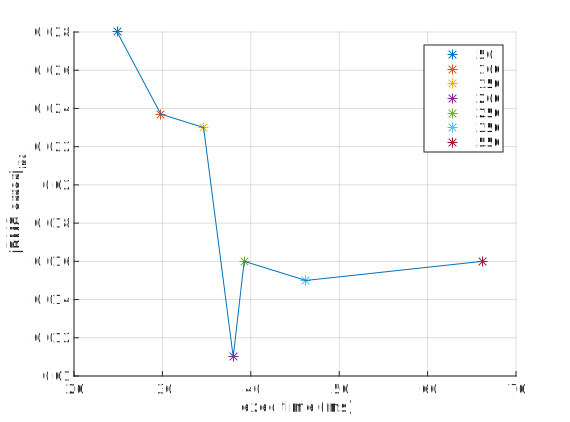
\includegraphics[width=0.7\linewidth]{figures/init_eps_delta_90th}
\caption{Error-delay curve for the FAST corner detector running on the Odroid U3}
\label{fig:fast}
\end{figure}

Fig.~\ref{fig:fastErrVsPower} shows the power consumption vs estimation error, which correlates well with Fig.~\ref{fig:fast}.
\begin{figure}[t]
	\centering
	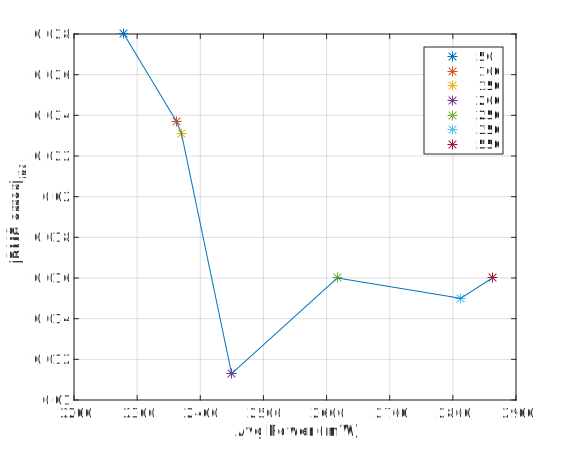
\includegraphics[width=0.7\linewidth]{figures/errVsPower}
	\caption{Error-delay curve for the FAST corner detector running on the Odroid U3}
	\label{fig:fastErrVsPower}
\end{figure}